\newpage
\chapter{Desenvolvimento}
\label{ch:desenvolvimento}

% \par Este capítulo irá detalhar como as novas funcionalidades foram desenvolvidas para o framework Esfinge Gamification.

%\par Como o Esfinge Gamification é utilizado por outros desenvolvedores, o projeto \textbf{DrawableNNAPI}\footnote{O projeto está disponível em: https://gitlab.com/django-livre/DrawRestfulAPI} foi desenvolvido a fim de identificar possíveis melhorias e/ou novas funcionalidades que poderiam ser aplicadas no framework.

%\section{Método \textit{getAllAchievements}}
%\par Foi criado um método para recuperar todos as conquistas por tipo, como a próxima listagem irá exibir, este método recebe como parâmetro uma classe que estenda a classe abstrata \textit{Achievement}, portanto uma conquista, a partir deste parâmetro as conquistas serão recuperadas. A utilidade deste método é o auxilio na criação de rankings e/ou a comparações entre todos os usuários.

\par Este capítulo detalha as soluções desenvolvidas para o problema citado na introdução do TG. Para que os novos recursos fossem adicionados ao Esfinge Gamification, foi necessário alterar seu fluxo de funcionamento exibido anteriormente na Figura \ref{fig:diagrama-funcionamento-gamification} a fim de adicionar os processos de autorização. Atualmente o \textit{framework} possui o fluxo de funcionamento da Figura \ref{fig:fluxo-atual}. 

\begin{figure}[H]
    \centering
    \caption{Fluxo de funcionamento atual do Esfinge Gamification}
    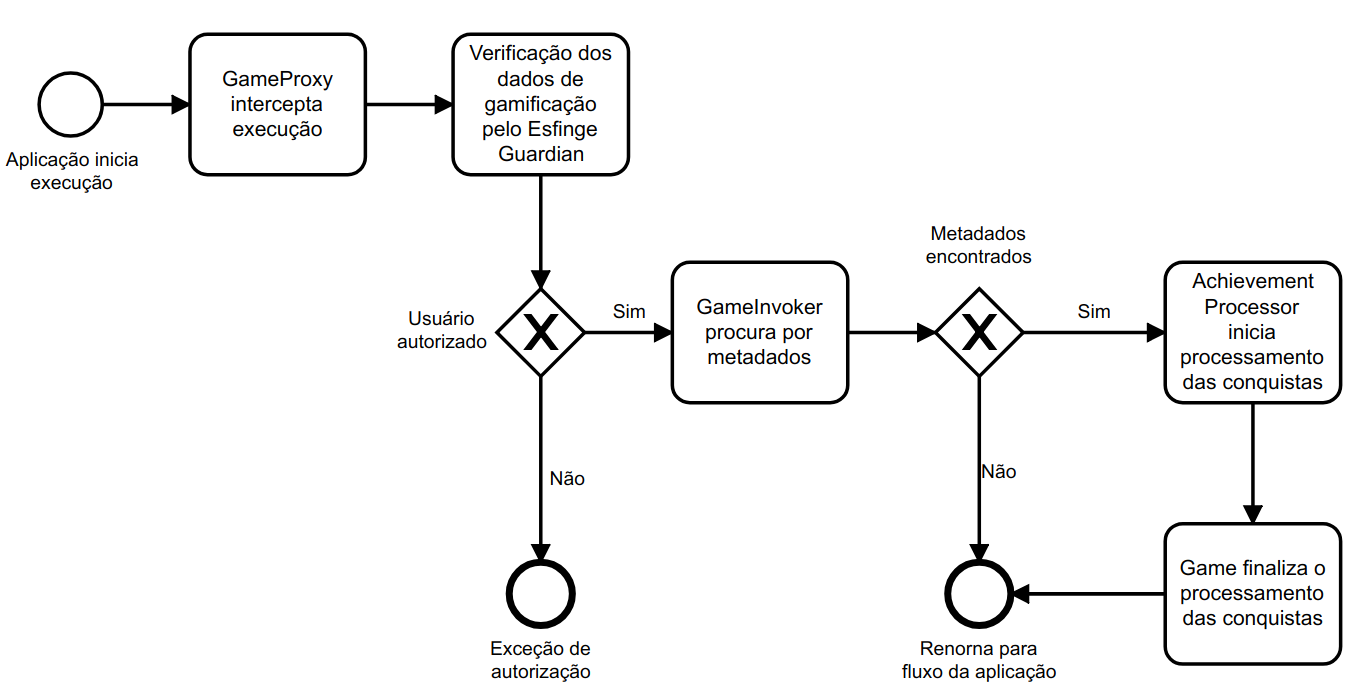
\includegraphics[scale=0.3]{src/imagens/cap3/fluxo-atual.png}
    \label{fig:fluxo-atual}
\end{figure}

\par Neste fluxo, aplicações em que o Esfinge Gamification foi configurado, são interceptadas via PD conforme já dito, porém o diferencial é que antes do fluxo de gamificação ser executado o Esfinge Guardian é invocado para que validações de autorização do usuário sejam realizadas. Na linha 9 da Figura \ref{fig:esfinge-proxy} um objeto que será interceptado pelo Esfinge Guardian é criado, e na linha 155 em que o método interceptado pelo PD do Esfinge Gamification é invocado, o objeto passado como parâmetro para a execução é o PD do Esfinge Guardian. Desta forma a responsabilidade de execução é passada para o Esfinge Guardian e as validações ocorrem de acordo com o diagrama de sequencia exibido na Figura \ref{fig:diagrama-funcionamento-guardian}.

\begin{figure}[H]
    \centering
    \caption{Criação do \textit{proxy} dinâmico do Esfinge Gamification}
    \begin{java}
public class GameProxy implements InvocationHandler {

    private Object encapsulated;
	private Object guardedObject; 
    
    private GameProxy(Object encapsulated) {
        this.encapsulated = encapsulated;
    	// tratativa de excecao omitida
    	this.guardedObject = AuthorizationContext.guardObject(encapsulated);
    	
    }

    public Object invoke(Object proxy, Method method, Object[] args) throws Throwable {
    	try {
        	Object returnValue = method.invoke(guardedObject, args);
        	GameInvoker gameInvoker = GameInvoker.getInstance();
        	gameInvoker.registerAchievment(encapsulated, method, args);
    
    	    return returnValue;
    	} catch (InvocationTargetException e) {
    	    throw e.getTargetException();
    	}
    }
    
    //metodo de criacao do proxy dinamico ja exibido foi omitido
}
    \end{java}
    \label{fig:esfinge-proxy}
    \fonte{Produção do autor}
\end{figure}

\par O diagrama de classes exibido na Figura \ref{fig:gamification-diagrama-classe-cap3} evidencia as mudanças feitas. Nele é possível verificar que a Classe \textit{GameProxy} agora possui dois objetos encapsulados, o objeto que foi recebido para criação do PD \textit{(encapsulated)} e o criado para ser interceptado pelo Esfinge Guardian \textit{(guardedObject)}.

\begin{landscape}
    \begin{figure}    \caption{Diagrama de classes atual Esfinge Gamification}
    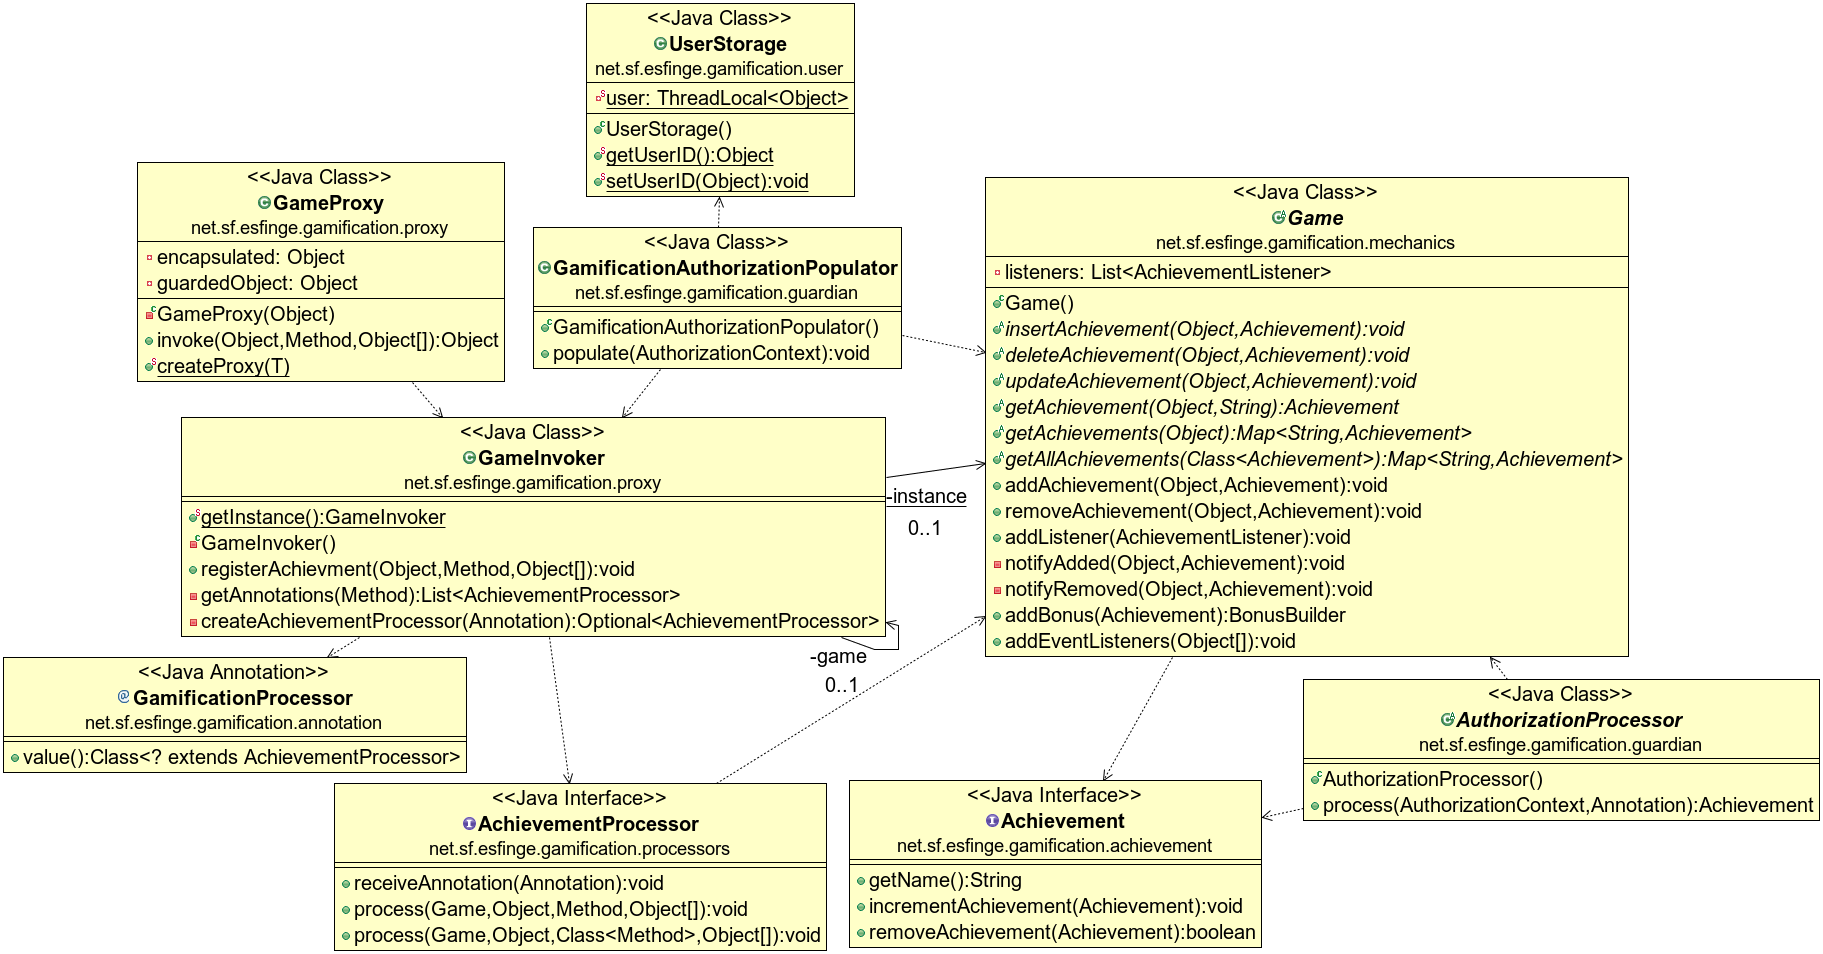
\includegraphics[scale=0.42]{src/imagens/cap3/gamification-class-diagram-cap3.png}
    \label{fig:gamification-diagrama-classe-cap3}
    \fonte{Produção do autor}
    \end{figure}
\end{landscape}

\par Durante o fluxo de execução do Esfinge Guardian (Figura \ref{fig:diagrama-funcionamento-guardian}), implementações da interface \textit{Populator} são procuradas para recuperação de informações necessárias para autorização. A implementação criada para recuperação dos dados de gamificação foi chamada de \textit{GamificationAuthorizationPopulator}, seu funcionamento é detalhado na Figura \ref{fig:bpmn-gamification-populator}. O método de configuração do \textit{Populator} escolhido foi via arquivo de configuração, portanto existe um arquivo chamado \textit{org.esfinge.guardian.populator.Populator} com o conteúdo \textit{net.sf.esfinge.gamification.guardian.GamificationAuthorizationPopulator} localizado no diretório \textit{META-INF/services}. 

\begin{image}
{0.5}
{src/imagens/cap3/bpmn-fluxo-gamification-populator.png}
{Fluxo de funcionamento \textit{GamificationAuthorizationPopulator}}
{fig:bpmn-gamification-populator}
{Produção do autor}
\end{image}

\par A classe \textit{Game} e o valor armazenado em \textit{UserStorage} são inseridos no contexto de autorização, pois com o valor armazenado em \textit{UserStorage} é possível identificar qual usuário terá o \textit{Achievement} recuperado, e com a classe \textit{Game} é possível recuperar o \textit{Achievement} do usuário. As anotações de segurança são inseridas no Esfinge Guardian para que estas sejam identificadas posteriormente, quando as implementações de \textit{Authorizers} forem executadas pelo \textit{framework} conforme Figura \ref{fig:diagrama-funcionamento-guardian}.

\par Para utilização das funcionalidades de autorização integradas, as anotações disponíveis no pacote \textit{net.sf.esfinge.gamification.annotation.auth} da Tabela \ref{tab:autorizacoes} foram criadas.

\begin{longtable}{|l|m{9cm}|}
\caption{Anotações de autorização desenvolvidas}\\
\hline
Anotação & Comportamento \\ \hline
\endfirsthead
\endhead
\begin{tabular}[c]{@{}l@{}}
@AllowPointGreaterThan,\\ @AllowPointLessOrEqualsThan,\\ @DenyPointLessOrEqualsThan, \\ @DenyPointGreaterThan
\end{tabular} & Estas anotações verificam se os pontos respeitam as restrições de maior ou menor igual a uma determinada quantidade definida na anotação para que a autorização seja concedida. \\ \hline
\begin{tabular}[c]{@{}l@{}}
@AllowRanking,\\
@AllowLevel,\\ 
@AllowRankingAndLevel,\\
@AllowRankingOrLevel,\\ 
@DenyLevel,\\
@DenyRanking,\\ 
@DenyRankingAndLevel,\\
@DenyRankingOrLevel
\end{tabular} & As anotações de \textit{Ranking} verificam as condições das propriedades ranking e level das conquistas, para permitir ou não o acesso a recursos. \\ \hline
@AllowTrophy, @DenyTrophy & Anotações de \textit{Thropy} permitem ou não que um usuário acesse o recurso. \\ \hline
@AllowReward, @DenyReward & Anotações de \textit{Reward} verificam se o usuário poderá ou não acessar um recurso com determinado \textit{Reward}.
\label{tab:autorizacoes}
\\ \hline
\end{longtable}

%\par A partir destas anotações é possível realizar o controle de acesso passando a responsabilidade para o Esfinge Guardian. 
\par Para cada anotação criada foi preciso implementar a interface \textit{Authorizer} conforme descrito anteriormente no capítulo \ref{ch:fundamentacao}. Na Figura \ref{fig:processo-autorizacao-gamification} é possível visualizar o processo realizado pelo Esfinge Guardian para verificar as informações de gamificação do usuário.

\begin{image}
{0.5}
{src/imagens/cap3/bpmn-authorizer.png}
{Processo de autorização baseado nas conquistas}
{fig:processo-autorizacao-gamification}
{Produção do autor}
\end{image}

%s Figuras \ref{fig:allow-trophy} e \ref{fig:allow-trophy-authorizer} a anotação @AllowTrophy e a classe AllowTrophyAuthorizer serão abordadas para melhor entendimento do que foi desenvolvido.

\par Todas as implementações de \textit{Authorizer} criadas estendem a classe abstrata \textit{AuthorizationProcessor} (Figura \ref{fig:authorization-processor}), que tem como objetivo principal a recuperação do \textit{Achievement} utilizado na autorização. É possível verificar nas linhas 5 e 6 que o \textit{Game} e o usuário inseridos no contexto de autorização pela classe \textit{GamificationAuthorizationPopulator} (Figura \ref{fig:bpmn-gamification-populator}) são utilizados nesta etapa, pois o \textit{Achievement} é buscado e recuperado com estas informações na linha 25.
\par Na linha 8 a anotação de autorização recebida é validada para que exceção \textit{NullPointerException} não ocorra em tempo de execução quando o tipo da anotação for recuperado via reflexão (linha 12). Como as implementações de \textit{Achievement} presentes no Esfinge Gamification devem possuir um método para recuperar seu nome (Figura \ref{fig:interface-achievement}), foi criada a definição programática "achievementName"\ para as anotações de segurança, isto é, toda anotação de segurança possui uma propriedade chamada "achievementName", possibilitando assim a recuperação do nome do \textit{Achievement} via reflexão, processo realizado nas linhas 16 e 17.

\begin{figure}[H]
    \centering
    \caption{Classe \textit{AuthorizationProcessor}}
    \begin{java}
public abstract class AuthorizationProcessor {

	public Achievement process(AuthorizationContext context, Annotation securityAnnotation) {
		
		Game game = (Game) context.getEnvironment().get("game");
		Object user = (Object) context.getResource().get("currentUser");

		if (Objects.isNull(securityAnnotation))
			throw new GamificationConfigurationException(
					"One security annotation it's necessary to validade this process");

		Class<? extends Annotation> annotationType = securityAnnotation.annotationType();
		String achiev = "";

		try {
			Method achievGetter = annotationType.getMethod("achievementName");
			achiev = (String) achievGetter.invoke(securityAnnotation);
		} catch (IllegalAccessException | IllegalArgumentException | InvocationTargetException | NoSuchMethodException
				| SecurityException invokeException) {
			throw new GamificationConfigurationException(
					"Achievement name property could not be found in annotation " + annotationType.getName(),
					invokeException);
		}

		Achievement achievement = game.getAchievement(user, achiev);

		return achievement;
	}
}
    \end{java}
    \label{fig:authorization-processor}
\end{figure}

\par Com essas implementações foi possível realizar o controle de acesso baseado em conquistas cumprindo os objetivos definidos.

\section{Visão geral}

\par Esta seção tem como objetivo explicar como o \textit{framework} deve ser usado. A Figura \ref{fig:hellow-world-gamification} realiza a configuração do Esfinge Gamification em um ambiente em que as notas podem ser atribuídas a usuários apenas por quem possuir o Ranking \textit{Avaliator} e o Level \textit{Master}.


\begin{figure}[H]
    \centering
    \caption{Configuração e utilização do \textit{framework}}
    \begin{java}
public class AuthorizationSample {

	public static void main(String[] args) {

		User user = new User();
		user.setClassroom("C12019");
		user.setRa("C1A252019");
		
		// Metodo de persistencia de conquistas escolhido foi o armazenamento de memoria
		Game game = new GameMemoryStorage();

		// Configuracao do Esfinge Gamification
		GameInvoker.getInstance().setGame(game);
		UserStorage.setUserID(user.getRa());

		// Cria um PD para ser interceptado
		Person pdUser = GameProxy.createProxy(user);

		pdUser.addNote(10.0);

	}
}
    \end{java}
    \label{fig:hellow-world-gamification}
    \fonte{Produção do autor}
\end{figure}

Neste exemplo o usuário atual tenta alterar seus pontos e recebe a exceção \textit{"Unauthorized Access"} do pacote \textit{org.esfinge.guardian.exception.AuthorizationException} devido a falta do \textit{Ranking} e do \textit{Level} necessários, a Figura \ref{fig:execao-configuracao} exibe a configuração realizada na classe \textit{User} para que a autorização seja monitorada pelo Esfinge Guardian.

\begin{figure}[H]
    \centering
    \caption{Configuração de segurança da classe \textit{User}}
    \begin{java}
public class User implements Person {

	private String classroom;
	private String ra;
	private List<Double> notes;

// constructor omitido
    
// Anotacao de configuracao
        @Override
	@AllowRankingAndLevel(achievementName = "Avaliator", level = "Master")
	public void addNote(Double note) {
		List<Double> notes = this.getNotes();
		Objects.requireNonNull(notes, "Notes can't be null");
		notes.add(note);
	}
	
// Getters and setters omitidos
}
    \end{java}
    \label{fig:execao-configuracao}
    \fonte{Produção do autor}
\end{figure}

\par Para que notas pudessem ser adicionadas pelo usuário seria necessário adicionar o \textit{Ranking} utilizado na regra de autorização descrita no inicio desta seção. O exemplo apresentado na Figura \ref{fig:autorizacao-ok} exibe um novo método criado para a atribuição desta autorização por meio da adição do \textit{Achievement} necessário.


\begin{figure}[H]
    \centering
    \caption{Interface \textit{Person}}
    \begin{java}
public interface Person {

	void addNote(Double note);

	@RankingsToUser(name = "Avaliator", level = "Master")
	void promotePerson();
}
    \end{java}
    \label{fig:autorizacao-ok}
\end{figure}

\par A única alteração feita para a adição das notas ser autorizada é a ordem das chamadas, como é possível observar na Figura \ref{fig:hellow-world-gamification-autorizada} onde o método \textit{promotePerson} é invocado na linha 18 antes da adição da nota.

\begin{figure}[H]
    \centering
    \caption{Operação autorizada pelo Esfinge Guardian}
    \begin{java}
public class AuthorizationSample {

	public static void main(String[] args) {

		User user = new User();
		user.setClassroom("C12019");
		user.setRa("C1A252019");
		
		Game game = new GameMemoryStorage();

	    Esfinge Gamification
		GameInvoker.getInstance().setGame(game);
		UserStorage.setUserID(user.getRa());

		Person pdUser = GameProxy.createProxy(user);
		
		// a anotacao neste metodo faz o usuario possuir o Achievement utilizado na regra de autorizacao
		pdUser.promotePerson();
		pdUser.addNote(10.0);

	}
}
    \end{java}
    \label{fig:hellow-world-gamification-autorizada}
\end{figure}